\chapter{HYDROGEN ATOM }
\section{Central Potential}
We are going to study the structure of the schrodinger equation for the particle of mass M moving in a spherically symmetric potential\\
 $V(\vec{r})=V(r)$,\\
which is also known as the central potential.\\
The time-independent Schrödinger equation for this particle, of momentum $-i \hbar \vec{\nabla}$ and position vector $r$, is
$$
\left[-\frac{\hbar^{2}}{2 M} \nabla^{2}+V(r)\right] \psi(\vec{r})=E \psi(\vec{r}) .
$$
Since the Hamiltonian is spherically symmetric, we are going to use the spherical coordinates $(r, \theta, \varphi)$ which are related to their Cartesian counterparts by
$$
x=r \sin \theta \cos \varphi, \quad y=r \sin \theta \sin \varphi, \quad z=r \cos \theta .
$$
The Laplacian $\nabla^{2}$ separates into a radial part $\nabla_{r}^{2}$ and an angular part $\nabla_{\Omega}^{2}$ as follows:
$$
\nabla^{2}=\nabla_{r}^{2}-\frac{1}{\hbar^{2} r^{2}}$$
 $$\nabla_{\Omega}^{2}=\frac{1}{r^{2}} \frac{\partial}{\partial r}\left(r^{2} \frac{\partial}{\partial r}\right)-\frac{1}{\hbar^{2} r^{2}}$$ $$\hat{\vec{L}}^{2}=\frac{1}{r} \frac{\partial^{2}}{\partial r^{2}} r-\frac{1}{\hbar^{2} r^{2}} \hat{\vec{L}}^{2}
$$
where $\hat{L}$ is the orbital angular momentum with
$$
\hat{\hat{L}}^{2}=-\hbar^{2}\left[\frac{1}{\sin \theta} \frac{\partial}{\partial \theta}\left(\sin \theta \frac{\partial}{\partial \theta}\right)+\frac{1}{\sin ^{2} \theta} \frac{\partial^{2}}{\partial \varphi^{2}}\right] .
$$
In spherical coordinates the Schrödinger equation therefore takes the form
$$
\left[-\frac{\hbar^{2}}{2 M} \frac{1}{r} \frac{\partial^{2}}{\partial r^{2}} r+\frac{1}{2 M r^{2}} \hat{\vec{L}}^{2}+V(r)\right] \psi(\vec{r})=E \psi(\vec{r}) .
$$
The first term of this equation can be viewed as the radial kinetic energy
$$
-\frac{\hbar^{2}}{2 M} \frac{1}{r} \frac{\partial^{2}}{\partial r^{2}} r=\frac{\hat{P}_{r}^{2}}{2 M},
$$
Now $\hat{\hat{L}}^{2}$ does not depends on r, it commute with both $\vec{V}(r)$ and the radial KE.Hence it also commute with the Hamiltonian H . In addition since $L_z$ commute with $\hat{\hat{L}}^{2}$, the three operators H,$\hat{\hat{L}}^{2}$, and $L_z$ mutually commute:
$$
\left[\hat{H}, \hat{\vec{L}}^{2}\right]=\left[\hat{H}, \hat{L}_{z}\right]=0 .
$$
Thus $\hat{H}, \hat{\vec{L}}^{2}$, and $\hat{L}_{z}$ have common eigenfunctions. We know that the simultaneous eigenfunctions of $\hat{\vec{L}}^{2}$ and $\hat{L}_{z}$ are given by the spherical harmonics $Y_{I m}(\theta, \varphi)$ :
$$
\begin{aligned}
&\hat{\vec{L}}^{2} Y_{l m}(\theta, \varphi)=l(l+1) \hbar^{2} Y_{l m}(\theta, \varphi), \\
&\hat{L}_{z} Y_{l m}(\theta, \varphi)=m \hbar Y_{l m}(\theta, \varphi) .
\end{aligned}
$$
Since the Hamiltonian is a sum of a radial part and an angular part, we can look for solutions that are products of a radial part and an angular part, where the angular part is simply the spherical harmonic $Y_{l m}(\theta, \varphi)$ :
$$
\psi(\vec{r})=\langle\vec{r} \mid n l m\rangle=\psi_{n l m}(r, \theta, \varphi)=R_{n l}(r) Y_{I m}(\theta, \varphi) .
$$
Note that the orbital angular momentum of a system moving in a central potential is conserved,it commutes with the Hamiltonian.

The radial wave function $R_{n l}(r)$ has yet to be found. The quantum number $n$ is introduced to identify the eigenvalues of $\hat{H}$ :
$$
\hat{H}|n l m\rangle=E_{n}|n l m\rangle
$$
Substituting $\psi_{n l m}(r, \theta, \varphi)$ into schrodinger equation and using the fact that $\psi_{n l m}(r, \theta, \varphi)$ is an eigenfunction of $\hat{\vec{L}}^{2}$ with eigenvalue $l(l+1) \hbar^{2}$, then dividing through by $R_{n l}(r) Y_{l m}(\theta, \varphi)$ and multiplying by $2 M r^{2}$, we end up with an equation where the radial and angular degrees of freedom are separated:
$$
\left[-\hbar^{2} \frac{r}{R_{n l}} \frac{\partial^{2}}{\partial r^{2}}\left(r R_{n l}\right)+2 M r^{2}(V(r)-E)\right]+\left[\frac{\hat{\vec{L}}^{2} Y_{l m}(\theta, \varphi)}{Y_{l m}(\theta, \varphi)}\right]=0 
$$
The terms inside the first square bracket are independent of $\theta$ and $\varphi$ and those of the second are independent of $r$. They must then be separately equal to constants and their sum equal to zero. The second square bracket is the the eigenvalue equation of $\hat{\vec{L}}^{2}$; hence it is equal to $l(l+1) \hbar^{2} .$ As for the first bracket, it must be equal to $-l(l+1) \hbar^{2}$; this leads to an equation known as the radial equation for a central potential:
$$
-\frac{\hbar^{2}}{2 M} \frac{d^{2}}{d r^{2}}\left(r R_{n l}(r)\right)+\left[V(r)+\frac{l(l+1) \hbar^{2}}{2 M r^{2}}\right]\left(r R_{n l}(r)\right)=E_{n}\left(r R_{n l}(r)\right) .
$$
Note that the above equation, which gives the energy levels of the system, does not depend on the azimuthal quantum number $m$. Thus, the energy $E_{n}$ is $(2 l+1)$-fold degenerate.
\section{Hydrogen Atom }
\begin{align*}
\intertext{Schrödinger's equation for the electron in three dimensions, which is what we must use for the hydrogen atom, is}
&\frac{\partial^{2} \psi}{\partial x^{2}}+\frac{\partial^{2} \psi}{\partial y^{2}}+\frac{\partial^{2} \psi}{\partial z^{2}}+\frac{2 m}{\hbar^{2}}(E-U) \psi=0
\intertext{The potential energy $U$ here is the electric potential energy
Electric potential}
U&=-\frac{e^{2}}{4 \pi \epsilon_{0} r}\\
\text{of a charge $-e$ when it is  }&\text{ the distance $r$ from another charge $+e$.}\\
\text{In spherical polar coordinates}&\text{ Schrödinger's equation is written}\\
\frac{1}{r^{2}} \frac{\partial}{\partial r}\left(r^{2} \frac{\partial \psi}{\partial r}\right)+\frac{1}{r^{2} \sin \theta} \frac{\partial}{\partial \theta}\left(\sin \theta \frac{\partial \psi}{\partial \theta}\right) &+\frac{1}{r^{2} \sin ^{2} \theta} \frac{\partial^{2} \psi}{\partial \phi^{2}}+\frac{2 m}{\hbar^{2}}(E-U) \psi=0\\
\text{Substituting  for the potential energy $U$ and}&\text{   multiplying the entire equation by $r^{2} \sin ^{2} \theta$, we obtain}\\
\intertext { Hydrogen atom }&\\ 
\sin ^{2} \theta \frac{\partial}{\partial r}\left(r^{2} \frac{\partial \psi}{\partial r}\right) &+\sin \theta \frac{\partial}{\partial \theta}\left(\sin \theta \frac{\partial \psi}{\partial \theta}\right) \\
+\frac{\partial^{2} \psi}{\partial \phi^{2}}&+\frac{2 m r^{2} \sin ^{2} \theta}{\hbar^{2}}\left(\frac{e^{2}}{4 \pi \epsilon_{0} r}+E\right) \psi=0
\end{align*}


Equation is the partial differential equation for the wave function $\psi$ of the electron in a hydrogen atom. Together with the various conditions $\psi$ must obey, namely that $\psi$ be normalizable and that $\psi$ and its derivatives be continuous and single-valued at each point $r, \theta, \phi$, this equation completely specifies the behavior of the electron.
\subsection{Seperation of Variables}
The advantage of writing Schrödinger's equation in spherical polar coordinates for the problem of the hydrogen atom is that in this form it may be separated into three independent equations, each involving only a single coordinate. Such a separation is possible here because the wave function $\psi(r, \theta, \phi)$ has the form of a product of three different functions: $R(r)$, which depends on $r$ alone; $\Theta(\theta)$ which depends on $\theta$ alone; and $\Phi(\phi)$, which depends on $\phi$ alone. Of course, we do not really know that this separation is possible yet, but we can proceed by assuming that\\
$$\psi(r, \theta, \phi)=R(r) \Theta(\theta) \Phi(\phi)$$
which we may write more simply as
$$
\psi=R \Theta \Phi
$$
we see that
$$
\begin{aligned}
\frac{\partial \psi}{\partial r} &=\Theta \Phi \frac{\partial R}{\partial r}=\Theta \Phi \frac{d R}{d r} \\
\frac{\partial \psi}{\partial \theta} &=R \Phi \frac{\partial \Theta}{\partial \theta}=R \Phi \frac{d \Theta}{d \theta} \\
\frac{\partial^{2} \psi}{\partial \phi^{2}} &=R \Theta \frac{\partial^{2} \Phi}{\partial \phi^{2}}=R \Theta \frac{d^{2} \Phi}{d \phi^{2}}
\end{aligned}
$$
When we substitute $R \Theta \Phi$ for $\psi$ in Schrödinger's equation for the hydrogen atom and divide the entire equation by $R \Theta \Phi$, we find that
$$
\begin{aligned}
\frac{\sin ^{2} \theta}{R} \frac{d}{d r}\left(r^{2} \frac{d R}{d r}\right)+\frac{\sin \theta}{\Theta} \frac{d}{d \theta}\left(\sin \theta \frac{d \Theta}{d \theta}\right) &+\frac{1}{\Phi} \frac{d^{2} \Phi}{d \phi^{2}} \\
&+\frac{2 m r^{2} \sin ^{2} \theta}{\hbar^{2}}\left(\frac{e^{2}}{4 \pi \epsilon_{0} r}+E\right)=0
\end{aligned}
$$
The third term  is a function of azimuth angle $\phi$ only, whereas the other terms are functions of $r$ and $\theta$ only.
Let us rearrange the equation to read
$$
\begin{aligned}
\frac{\sin ^{2} \theta}{R} \frac{d}{d r}\left(r^{2} \frac{d R}{d r}\right)+\frac{\sin \theta}{\Theta} \frac{d}{d \theta} &\left(\sin \theta \frac{d \Theta}{d \theta}\right) \\
&+\frac{2 m r^{2} \sin ^{2} \theta}{\hbar^{2}}\left(\frac{e^{2}}{4 \pi \epsilon_{0} r}+E\right)=-\frac{1}{\Phi} \frac{d^{2} \Phi}{d \phi^{2}}
\end{aligned}
$$
This equation can be correct only if both sides of it are equal to the same constant, since they are functions of different variables. As we shall see, it is convenient to call this constant $m_{l}^{2}$. The differential equation for the function $\phi$ is the refore
$$
-\frac{1}{\Phi} \frac{d^{2} \Phi}{d \phi^{2}}=m_{l}^{2}
$$
Next we substitute $m_{l}^{2}$ for the right-hand side the last equation and divide the entire equation by $\sin ^{2} \theta$, and rearrange the various terms, which yields
$$
\frac{1}{R} \frac{d}{d r}\left(r^{2} \frac{d R}{d r}\right)+\frac{2 m r^{2}}{\hbar^{2}}\left(\frac{e^{2}}{4 \pi \epsilon_{0} r}+E\right)=\frac{m_{l}^{2}}{\sin ^{2} \theta}-\frac{1}{\Theta \sin \theta} \frac{d}{d \theta}\left(\sin \theta \frac{d \Theta}{d \theta}\right)
$$
Again we have an equation in which different variables appear on each side, requiring that both sides be equal to the same constant. This constant is called $l(l+1)$, once more for reasons that will be apparent later. The equations for the functions $\Theta$ and $R$ are therefore\\
$$\begin{gathered}
\frac{m_{l}^{2}}{\sin ^{2} \theta}-\frac{1}{\Theta \sin \theta} \frac{d}{d \theta}\left(\sin \theta \frac{d \Theta}{d \theta}\right)=l(l+1) \\
\frac{1}{R} \frac{d}{d r}\left(r^{2} \frac{d R}{d r}\right)+\frac{2 m r^{2}}{\hbar^{2}}\left(\frac{e^{2}}{4 \pi \epsilon_{0} r}+E\right)=l(l+1)
\end{gathered}$$
Equation for $\Phi$ $$\frac{d^{2} \Phi}{d \phi^{2}}+m_{l}^{2} \Phi=0$$
Equation
for $\boldsymbol{\theta}$
$$\frac{1}{\sin \theta} \frac{d}{d \theta}\left(\sin \theta \frac{d \Theta}{d \theta}\right)+\left[l(l+1)-\frac{m_{l}^{2}}{\sin ^{2} \theta}\right] \Theta=0$$
Equation
for $R$
$$\frac{1}{r^{2}} \frac{d}{d r}\left(r^{2} \frac{d R}{d r}\right)+\left[\frac{2 m}{\hbar^{2}}\left(\frac{e^{2}}{4 \pi \epsilon_{0} r}+E\right)-\frac{l(l+1)}{r^{2}}\right] R=0$$
\subsection{Quantum Numbers}
\textbf{Magnetic Quantum Number}
$$\Phi(\phi)=A e^{i m_{l} \phi}$$
As we know, one of the conditions that a wave function-and hence $\Phi$, which is a component of the complete wave function $\psi$-must obey is that it have a single value at a given point in space.We konw that $\phi$ and $\phi+2 \pi$ both identify the same meridian plane. Hence it must be true that $\Phi(\phi)=$ $\Phi(\phi+2 \pi)$, or
$$A e^{i m_{l} \phi}=A e^{i m_{l}(\phi+2 \pi)}$$
which can happen only when $m_{l}$ is 0 or a positive or negative integer $(\pm 1$, $\pm 2, \pm 3$....). The constant $m_{l}$ is known as the magnetic quantum number of the hydrogen atom.\\
The differential equation for $\Theta(\theta)$, has a solution provided that the constant $l$ is an integer equal to or greater than $\left|m_{l}\right|$, the absolute value of $m_{l}$. This requirement can be expressed as a condition on $m_{l}$ in the form
$$
m_{l}=0, \pm 1, \pm 2, \ldots, \pm l
$$
The constant $l$ is known as the \textbf{orbital quantum number}\\
An atomic electron that possesses angular momentum interacts with an external magnetic field $\mathbf{B}$. The magnetic quantum number $m_{l}$ specifies the direction of $\mathbf{L}$ by determining the component of $\mathbf{L}$ in the field direction. This phenomenon is often referred to as space quantization.

If we let the magnetic-field direction be parallel to the $z$ axis, the component of $\mathbf{L}$ in this direction is
Space quantization $$L_{z}=m_{l} \hbar \quad m_{l}=0, \pm 1, \pm 2, \ldots, \pm l$$
The possible values of $m_{l}$ for a given value of $l$ range from $+l$ through 0 to $-l$, so that the number of possible orientations of the angular-momentum vector $\mathbf{L}$ in a magnetic field is $2 l+1$. When $l=0, L_{z}$ can have only the single value of 0 ; when $l=1, L_{z}$ may be $\hbar, 0$, or $-\hbar$; when $l=2, L_{z}$ may be $2 \hbar, \hbar, 0,-\hbar$, or $-2 \hbar ;$ and so on.\\
\begin{figure}[H]
	\centering
	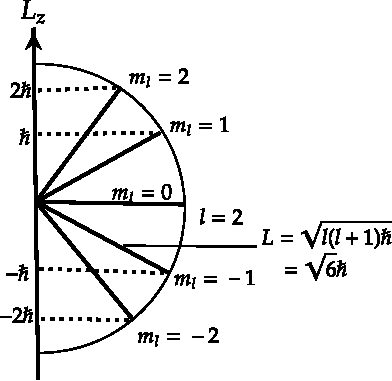
\includegraphics[height=5.5cm,width=6cm]{jamshi 6-crop}
	\caption{Space quantization of orbital angular momentum with (l=2)}
	\label{}
\end{figure}
\subsubsection{Orbital Quantum Mumber}
Electron angular momenta 
$$
L=\sqrt{l(l+1)} \hbar
$$
momentum
With the orbital quantum number $l$ restricted to the values
$$
l=0,1,2, \ldots,(n-1)
$$
The electron can have only the angular momenta $L$ specified by $
L=\sqrt{l(l+1)} \hbar
$, Like total energy E, angular momentum is both conserved and quantized. The quantity
$$
\hbar=\frac{h}{2 \pi}=1.054 \times 10^{-34} \mathrm{~J} \cdot \mathrm{s}
$$
is thus the natural unit of angular momentum.
\subsubsection{Designation of Angular-Momentum States}
It is customary to specify electron angular-momentum states by a letter, with $s$ corresponding to $l=0, p$ to $l=1$, and so on, according to the following scheme:\\\\
$\begin{array}{rlllllll}
	l=0 & 1 & 2 & 3 & 4 & 5 & 6 & \ldots \\
	s & p & d & f & g & h & i & \ldots
\end{array}$\\
$\begin{aligned}
	&\text { Table of Atomic Electron States }\\
	&\begin{array}{lcccccc}
		\hline & I=0 & I=1 & I=2 & I=3 & I=4 & I=5 \\
		\hline n=1 & 1 s & & & & & \\
		n=2 & 2 s & 2 p & & & & \\
		n=3 & 3 s & 3 p & 3 d & & & \\
		n=4 & 4 s & 4 p & 4 d & 4 f & & \\
		n=5 & 5 s & 5 p & 5 d & 5 f & 5 g & \\
		n=6 & 6 s & 6 p & 6 d & 6 f & 6 g & 6 h \\
		\hline
	\end{array}
\end{aligned}$\\\\
\textbf{Principal Quantum Number}\\
 For the radial part $R(r)$ of the hydrogenatom wave function $\psi$ also requires that a certain condition be fulfilled. This condition is that $E$ be positive or have one of the negative values $E_{n}$ (signifying that the electron is bound to the atom) specified by
$$
E_{n}=-\frac{m e^{4}}{32 \pi^{2} \epsilon_{0}^{2} \hbar^{2}}\left(\frac{1}{n^{2}}\right)=\frac{E_{1}}{n^{2}} \quad n=1,2,3, \ldots
$$
Another condition that must be obeyed in order to solve radial equation is that $n$, known as the principal quantum number, must be equal to or greater than $l+1$. This requirement may be expressed as a condition on $l$ in the form
$$
l=0,1,2, \ldots,(n-1)
$$
Hence we may tabulate the three quantum numbers $n, l$, and $m$ together with their permissible values as follows:\\
$$\begin{array}{lc}
	\text { Principal quantum number } & n=1,2,3, \ldots \\
	\text { Orbital quantum number } & l=0,1,2, \ldots,(n-1) \\
	\text { Magnetic quantum number } & m_{l}=0, \pm 1, \pm 2, \ldots, \pm l
\end{array}$$
To exhibit the dependence of $R, \Theta$, and $\Phi$ upon the quantum numbers $n, l, m$, we may write for the electron wave functions of the hydrogen atom
$$
\psi=R_{n l} \Theta_{l m_{l}} \Phi_{m_{l}}
$$
\subsection{Normalized Wavefunction of the Hydrogen Atom for N=1,2,3.}
{ \renewcommand*{\arraystretch}{2.5}
$\begin{array}{|c|c|c|c|c|c|c|}
	\hline n & l & m_{l} & \Phi(\phi) & \theta(\theta) & R(r) & \psi(r, \theta, \phi) \\
	\hline 1 & 0 & 0 & \frac{1}{\sqrt{2 \pi}} & \frac{1}{\sqrt{2}} & \frac{2}{a_{0}^{3 / 2}} e^{-r / a_{0}} & \frac{1}{\sqrt{\pi} a_{0}^{3 / 2}} e^{-r / a_{0}} \\
	2 & 0 & 0 & \frac{1}{\sqrt{2 \pi}} & \frac{1}{\sqrt{2}} & \frac{1}{2 \sqrt{2} a_{0}^{3 / 2}}\left(2-\frac{r}{a_{0}}\right) e^{-r / 2 a_{0}} & \frac{1}{4 \sqrt{2 \pi} a_{0}^{3 / 2}}\left(2-\frac{r}{a_{0}}\right) e^{-r / 2 a_{0}} \\
	2 & 1 & 0 & \frac{1}{\sqrt{2 \pi}} & \frac{\sqrt{6}}{2} \cos \theta & \frac{1}{2 \sqrt{6} a_{0}^{3 / 2}} \frac{r}{a_{0}} e^{-r / 2 a_{0}} & \frac{1}{4 \sqrt{2 \pi} a_{0}^{3 / 2}} \frac{r}{a_{0}} e^{-r / 2 a_{0}} \cos \theta \\
	2 & 1 & \pm 1 & \frac{1}{\sqrt{2 \pi}} e^{\pm i \phi} & \frac{\sqrt{3}}{2} \sin \theta & \frac{1}{2 \sqrt{6} a_{0}^{3 / 2}} \frac{r}{a_{0}} e^{-r / 2 a_{0}} & \frac{1}{8 \sqrt{\pi} a_{0}^{3 / 2}} \frac{r}{a_{0}} e^{-r / 2 a_{0}} \sin \theta e^{\pm i \phi}\\
	3&0&0&\frac{1}{\sqrt{2 \pi}}& \frac{1}{\sqrt{2}}&\frac{2}{81 \sqrt{3} a_{0}^{3 / 2}}\left(27-18 \frac{r}{a_{0}}+2 \frac{r^{2}}{a_{0}^{2}}\right) e^{-r / 3 a_{0}} &\frac{1}{81 \sqrt{3 \pi} a_{0}^{3 / 2}}\left(27-18 \frac{r}{a_{0}}+2 \frac{r^{2}}{a_{0}^{2}}\right) e^{-r / 3 a_{0}}\\
	3& 1&  0 &\frac{1}{\sqrt{2 \pi}} & \frac{\sqrt{6}}{2} \cos \theta & \frac{4}{81 \sqrt{6} a_{0}^{3 / 2}}\left(6-\frac{r}{a_{0}}\right) \frac{r}{a_{0}} e^{-r / 3 a_{0}} &\frac{\sqrt{2}}{81 \sqrt{\pi} a_{0}^{3 / 2}}\left(6-\frac{r}{a_{0}}\right) \frac{r}{a_{0}} e^{-r / 3 a_{0}} \cos \theta\\
	3 &1 & \pm 1 & \frac{1}{\sqrt{2 \pi}} e^{\pm i \phi} &\frac{\sqrt{3}}{2} \sin \theta & \frac{4}{81 \sqrt{6} a_{0}^{3 / 2}}\left(6-\frac{r}{a_{0}}\right) \frac{r}{a_{0}} e^{-r / 3 a_{0}} & \frac{1}{81 \sqrt{\pi} a_{0}^{3 / 2}}\left(6-\frac{r}{a_{0}}\right) \frac{r}{a_{0}} e^{-r / 3 a_{0}} \sin \theta e^{\pm i \phi}\\
	3&2&0 & \frac{1}{\sqrt{2 \pi}} & \frac{\sqrt{10}}{4}\left(3 \cos ^{2} \theta-1\right) & \frac{4}{81 \sqrt{30} a_{0}^{3 / 2}} \frac{r^{2}}{a_{0}^{2}} e^{-r / 3 a_{0}} & \frac{1}{81 \sqrt{6 \pi} a_{0}^{3 / 2}} \frac{r^{2}}{a_{0}^{2}} e^{-r / 3 a_{0}}\left(3 \cos ^{2} \theta-1\right)\\
	3 & 2 & \pm 1 & \frac{1}{\sqrt{2 \pi}} e^{\pm i \phi} & \frac{\sqrt{15}}{2} \sin \theta \cos \theta & \frac{4}{81 \sqrt{30} a_{0}^{3 / 2}} \frac{r^{2}}{a_{0}^{2}} e^{-r / 3 a_{0}} & \frac{1}{81 \sqrt{\pi} a_{0}^{3 / 2}} \frac{r^{2}}{a_{0}^{2}} e^{-r / 3 a_{o}} \sin \theta \cos \theta e^{\pm i \phi}\\
	3 & 2 &\pm 2 & \frac{1}{\sqrt{2 \pi}} e^{\pm 2 i \phi} & \frac{\sqrt{15}}{4} \sin ^{2} \theta&\frac{4}{81 \sqrt{30} a_{0}^{3 / 2}} \frac{r^{2}}{a_{0}^{2}} e^{-r / 3 a_{0}} & \frac{1}{162 \sqrt{\pi} a_{0}^{3 / 2}} \frac{r^{2}}{a_{0}^{2}} e^{-r / 3 a_{0}} \sin ^{2} \theta e^{\pm 2 i \phi}
\\	\hline
\end{array}$}
\subsection{Electron Probability Density}
The probability density $|\psi|^{2}$ that corresponds to the electron wave function $\psi=R \Theta \Phi$ in the hydrogen atom is
|$$\psi|^{2}=|\mathrm{R}|^{2}|\Theta|^{2}|\Phi|^{2}$$
we see that the azimuthal wave function is given by
$$
\Phi(\phi)=A e^{i m_{\ell} \phi}
$$
The azimuthal probability density $|\Phi|^{2}$ is therefore
$$
|\Phi|^{2}=\Phi^{*} \Phi=A^{2} e^{-i m_{1} \phi} e^{i m_{1} \phi}=A^{2} e^{0}=A^{2}
$$
The likelihood of finding the electron at a particular azimuth angle $\phi$ is a constant that does not depend upon $\phi$ at all. The electron's probability density is symmetrical about the $z$ axis regardless of the quantum state it is in, and the electron has the same chance of being found at one angle $\phi$ as at another.\\
\par The probability density of the electron at the point $r, \theta, \phi$ is proportional to $|\psi|^{2}$, but the actual probability of finding it in the infinitesimal volume element $d V$ there is $|\psi|^{2} d V$. In spherical polar coordinates  $\begin{aligned} d V &=(d r)(r d \theta)(r \sin \theta d \phi) \\ &=r^{2} \sin \theta d r d \theta d \phi \end{aligned}$\\
As $\Theta$ and $\Phi$ are normalized functions, the actual probability $P(r) d r$ of finding the electron in a hydrogen atom somewhere in the spherical shell between $r$ and $r+d r$ from the nucleus is
$$
\begin{aligned}
P(r) d r &=r^{2}|R|^{2} d r \int_{0}^{\pi}|\Theta|^{2} \sin \theta d \theta \int_{0}^{2 \pi}|\Phi|^{2} d \phi \\
&=r^{2}|R|^{2} d r
\end{aligned}
$$
\begin{figure}[H]
	\centering
	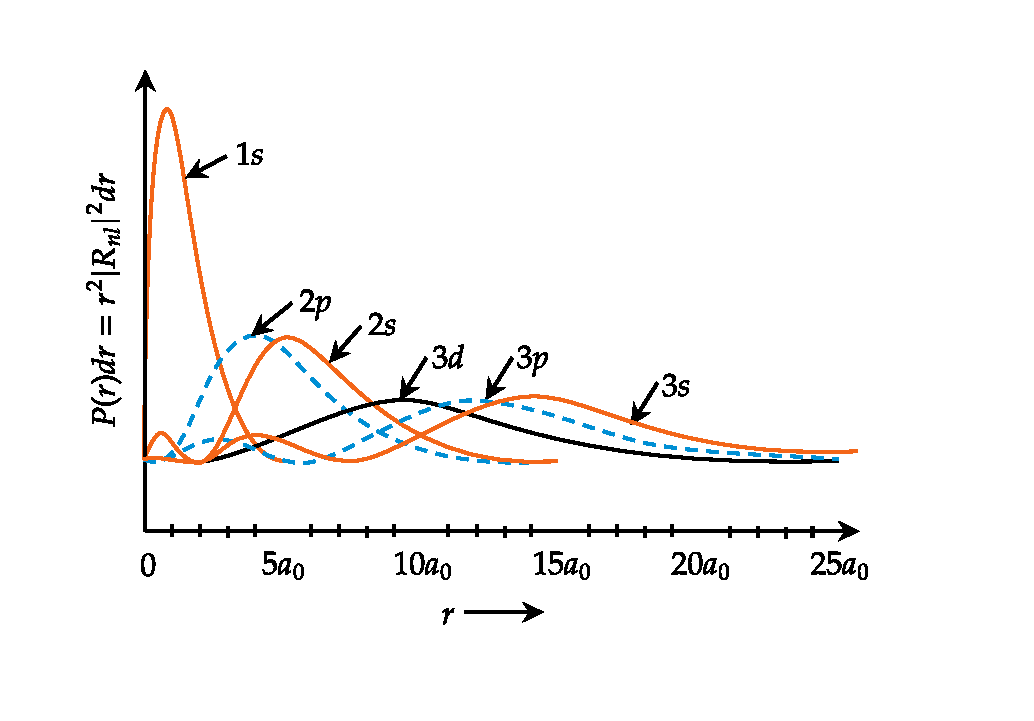
\includegraphics[height=7.5cm,width=10.5cm]{diagram-20220115(7)}
	\caption{The probability of finding the electron in a hydrogen atom at a distance between $r$ and $r+d r$ from the nucleus for the quantum states.}
\end{figure}
\subsection{ Degeneracy of Hydrogen Atom}
If spin of the electron is not included then degeneracy of atom is $\sum_{i=0}^{n-1}(2 l+1)=n^{2}$\\
If spin of the electron is included then degeneracy of atom is $2 \sum_{l=0}^{n-1}(2 l+1)=2 n^{2}$

\begin{exercise}
	$\text { Verify that the average value of } 1 / r \text { for a } 1 \text { s electron in the hydrogen atom is } 1 / a_{0} \text {. }$
\end{exercise}
\begin{answer}
The wave function of a ls electron is,
$$
\psi=\frac{e^{-r / a_{0}}}{\sqrt{\pi} a_{0}^{3 / 2}}
$$
Since $d V=r^{2} \sin \theta d r d \theta d \phi$ we have for the expectation value of $1 / r$
$$
\begin{aligned}
\left\langle\frac{1}{r}\right\rangle &=\int_{0}^{\infty}\left(\frac{1}{r}\right)|\psi|^{2} d V \\
&=\frac{1}{\pi a_{0}^{3}} \int_{0}^{\infty} r e^{-2 r / a_{0}} d r \int_{0}^{\pi} \sin \theta d \theta \int_{0}^{2 \pi} d \phi
\end{aligned}
$$
The integrals have the respective values
$$
\begin{gathered}
\int_{0}^{\infty} r e^{-2 r / a_{0}} d r=\left[\frac{a_{0}^{2}}{4} e^{-2 r / a_{0}}-\frac{r}{2} e^{-2 r / a_{0}}\right]_{0}^{\infty}=\frac{a_{0}^{2}}{4} \\
\int_{0}^{\pi} \sin \theta d \theta=[-\cos \theta]_{0}^{\pi}=2 \\
\int_{0}^{2 \pi} d \phi=[\phi]_{0}^{2 \pi}=2 \pi \\
\left\langle\frac{1}{r}\right\rangle=\left(\frac{1}{\pi a_{0}^{3}}\right)\left(\frac{a_{0}^{2}}{4}\right)(2)(2 \pi)=\frac{1}{a_{0}}
\end{gathered}
$$	
\end{answer}
\begin{exercise}
 Show that the most probable distance by the electron from the nucleus in the ground state of hydrogen atom is equal to the Bohr's radius.
\end{exercise}
\begin{answer}
For the ground state of hydrogen atom, $n=1, \ell=0$ and $m=0$. Hence the ground state wave function is,
$$
\psi_{1,0,0}=\left(\frac{1}{\pi a_{0}^{3}}\right)^{1 / 2} e^{-r / a_{0}}
$$
Since, the wave function is independent of $\theta$ and $\phi$, therefore,\\
Radial probability density $=P(r)=\left|\psi_{100}\right|^{2} 4 \pi r^{2}=\frac{4}{a_{0}^{3}} e^{-2 r / a_{0}} r^{2}$
For most probable distance, $P(r)$ is to be the maximum
$$
\frac{d P}{d r}=\frac{4}{a_{0}^{3}}\left[r^{2}\left(-\frac{2}{a_{0}}\right) e^{-2 r / a_{0}}+2 r e^{-2 r / a_{0}}\right]=0 \Rightarrow r=a_{0}
$$
Thus the most probable distance of the electron from the nucleus of hydrogen atom in the ground state is equal tothe Bohr radius $\left(a_{0}\right)$.	
\end{answer}
\begin{exercise}
 If the ground state wave function for the hydrogen atom is
	$$
	\psi=\frac{1}{\sqrt{\pi}} \frac{1}{a_{0}^{3 / 2}} e^{-r / a_{0}}
	$$
	show that average distance of the electron from the nucleus is $1.5 \mathrm{a}_{0}$.
\end{exercise}
\begin{answer}
	We have the average distance of the electron from the hydrogen nucleus in the ground state is,
	$$
	\begin{aligned}
	\langle r\rangle &=\int_{0}^{\infty} \psi^{*} \hat{r} \psi d r=\int_{0}^{\infty} \frac{1}{\sqrt{\pi}} \frac{1}{a_{0}^{3 / 2}} e^{-r / a_{0}} r \frac{1}{\sqrt{\pi}} \frac{1}{a_{0}^{3 / 2}} e^{-r / a_{0}} d \tau \\
	&=\frac{1}{\pi a_{0}^{3}} \int_{0}^{\infty} r e^{-2 r / a_{0}} r^{2} \sin \theta d r d \theta d \phi
	\end{aligned}
	$$
	Using the standard integral $\int_{0}^{\infty} e^{-a x} x^{n} d x=\frac{n !}{a^{n+1}}$, we get
	$$
	\langle r\rangle=\frac{1}{\pi a_{0}^{3}} \int_{0}^{\infty} r^{3} e^{-2 r / a_{0}} d r \int_{0}^{\pi} \sin \theta d \theta \int_{0}^{2 \pi} d \phi=\frac{1}{\pi a_{0}^{3}} \times \frac{3 !}{\left(2 / a_{0}\right)^{4}} \times 2 \times 2 \pi
	$$
	Therefore, $\langle r\rangle=\frac{3}{2} a_{0}=1.5 a_{0}$
\end{answer}
\begin{exercise}
	 What is the expectation value of the knetice nergy $\left(E^{2}\right)$ of the electron in the 1s state of the hydrogen atom?
\end{exercise}
\begin{answer}
	The expectation value of the kinetic energy is,
	$$
	\left\langle E_{k}\right\rangle=\int_{\tau} \psi_{1,0,0}^{*} \hat{E}_{k} \psi_{1,0,0} d \tau=\int_{0}^{\infty} \int_{0}^{\pi} \int_{0}^{2 \pi} \psi_{1,0,0} \hat{E}_{k} \psi_{1,0,0} r^{2} \sin \theta d r d \theta d \phi
	$$
	But, $\quad \vec{E}_{k}=-\frac{\hbar^{2}}{2 m} \nabla^{2}=-\frac{\hbar^{2}}{2 m}\left[\frac{1}{r^{2}} \frac{\partial}{\partial r} r^{2} \frac{\partial}{\partial r}+\frac{1}{r^{2} \sin \theta} \frac{\partial}{\partial \theta} \sin \theta \frac{\partial}{\partial \theta}+\frac{1}{r^{2} \sin ^{2} \theta} \frac{\partial^{2}}{\partial \phi^{2}}\right]$\\
	Since $\psi_{1,0,0}$ depends on $r$ only, the terms in $\frac{\partial}{\partial \theta}$ and $\frac{\partial}{\partial \phi}$ are zero.\\
	$$\left\langle E_{k}\right\rangle=-\frac{\hbar^{2}}{2 m} \cdot 4 \pi\left(\frac{1}{\sqrt{\pi} a_{0}^{3}}\right)^{2} \int_{0}^{\infty} e^{-r / a_{0}} \times\left\{\left(\frac{\partial^{2}}{\partial r^{2}}+\frac{2}{r} \frac{\partial}{\partial r}\right) e^{-r / a_{0}}\right\} r^{2} d r$$
	$$\begin{aligned}
		&=-\frac{\hbar^{2}}{2 m} \frac{4}{a_{0}^{3}} \int_{0}^{\infty}\left(\frac{1}{a_{0}^{2}}-\frac{2}{r a_{0}}\right) e^{-2 r / a_{0}} r^{2} d r \\
		&=-\frac{2 \hbar^{2}}{m a_{0}^{3}}\left[\frac{1}{a_{0}^{2}} \int_{0}^{\infty} r^{2} e^{-2 r / a_{0}} d r-\frac{2}{a_{0}} \int_{0}^{\infty} r e^{-2 r / a_{0}} d r\right] \\
		&=-\frac{2 \hbar^{2}}{m a_{0}^{3}}\left[\frac{1}{a_{0}^{2}} \frac{2}{\left(2 / a_{0}\right)^{3}}-\frac{2}{a_{0}} \frac{1}{\left(2 / a_{0}\right)^{2}}\right]=\frac{2 \hbar^{2}}{m a_{0}^{3}} \cdot \frac{a_{0}}{4}
	\end{aligned}$$
	$\text { Therefore, }\left\langle E_{k}\right\rangle=\frac{\hbar^{2}}{2 m a_{0}^{3}}=\frac{\hbar^{2}}{2 m}\left(\frac{m e^{2}}{\hbar^{2}}\right)=\frac{m e^{4}}{2 \hbar^{2}}$
\end{answer}
\begin{exercise}
 Estimate the uncertainity in the radial position of the electron in the ground state of hydrogen atom.
\end{exercise}
\begin{answer}
	\begin{align*}
	\text{For ground state}\\
	\langle r \rangle &=\frac{4}{a_0^3}	\int_{0}^{\infty} r^3 e^{\frac{-2r}{a_0}}dr=\frac{3a_0}{2}\\
	\langle r^2 \rangle &=\frac{4}{a_0^3}	\int_{0}^{\infty} r^4 e^{\frac{-2r}{a_0}}dr=3a_0^2\\
	\text{uncertainity in the }&\text{radial position of the particle will be }\\
	\Delta r&=\sqrt{\langle r^2 \rangle-\langle r \rangle^2}=\frac{\sqrt{3}}{2}a_0
	\end{align*}
\end{answer}
\begin{exercise}
	Find the positions of maxima of the radial probability curves for 1s,2s,2p and 3d orbitals of the hydrogen like atom 
\end{exercise}
\begin{answer}
	\begin{align*}
\text{	The radial probability density}\\
P_{nl}&=r^2|R_{nl}|^2\\
R_{10}&=Constant \times e^{-Zr/a_0}\\
R_{21}&=Constant \times e^{-Zr/2a_0}\\
R_{32}&=Constant \times e^{-Zr/3a_0}\\
\text{$P_{nl}$ will be maximum when $\frac{dP_{nl}}{dr}$}&=\text{$0$ hence }\\
\frac{dP_{10}}{dr}&=0 \implies C(2r-\frac{2Zr^2}{a_0})e^{\frac{-2Zr}{a_0}}=0\\
\implies r&=\frac{a_0}{Z}\\
\frac{dP{21}}{dr}&=0\implies C(4r^3-\frac{Zr^4}{a_0})e^{\frac{-Zr}{a_0}}=0\\
\implies r&=\frac{4a_0}{Z}\\
\text{Similarly }\frac{dP_{32}}{dr}&=0\implies r=\frac{9a_0}{2}\\
\text{In general }r_{max}&=\frac{n^2a_0}{2}
	\end{align*}
\end{answer}
\begin{exercise}
	 At time $t=0$, the wave function for the hydrogen atom is
	$$
	\psi(r, 0)=\frac{1}{\sqrt{10}}\left(2 \psi_{100}+\psi_{210}+\sqrt{2} \psi_{211}+\sqrt{3} \psi_{21,-1}\right)
	$$
	where the subscripts are values of the quantum numbers $n, l, m$. (i) What is the expectation value for the energy of the system? (ii) What is the probability of finding the system with $l=1, m=1$ ? .
\end{exercise}
\begin{answer}
	Expectation value $=\langle E \rangle =\langle \psi |H|\psi\rangle$\\
$$=\frac{1}{10}\left\langle \left(2 \psi_{100}+\psi_{210}+\sqrt{2} \psi_{211}+\sqrt{3} \psi_{21,-1}\right)|H|\left(2 \psi_{100}+\psi_{210}+\sqrt{2} \psi_{211}+\sqrt{3} \psi_{21,-1}\right)\right\rangle $$
$$=\frac{1}{10}\left\langle \left(2 \psi_{100}+\psi_{210}+\sqrt{2} \psi_{211}+\sqrt{3} \psi_{21,-1}\right)|\left(2E_1 \psi_{100}+E_2\psi_{210}+\sqrt{2} E_2\psi_{211}+\sqrt{3}E_2 \psi_{21,-1}\right)\right\rangle $$
$$=\frac{1}{10}\left( 4E_1+E_2+2E_2+3E_2\right) =\frac{1}{10}\left[ 4E_1+6E_2\right] $$
$$E_1=-13.6eV \quad E_2=-3.4eV$$
$$\langle E \rangle=-74.8eV$$
\end{answer}



\newpage
\begin{abox}
	Practice set 1
	\end{abox}
\begin{enumerate}
	\begin{minipage}{\textwidth}
		\item The energy levels of the non-relativistic electron in a hydrogen atom (i.e. in a Coulomb potential $V(r) \propto-1 / r$ ) are given by $E_{n l m} \propto-1 / n^{2}$, where $n$ is the principal quantum number, and the corresponding wave functions are given by $\psi_{n l m}$, where $l$ is the orbital angular momentum quantum number and $m$ is the magnetic quantum number. The spin of the electron is not considered. Which of the following is a correct statement?
		\exyear{NET JUNE 2011}
	\end{minipage}
	\begin{tasks}(1)
		\task[\textbf{A.}] There are exactly $(2 l+1)$ different wave functions $\psi_{n l m}$, for each $E_{n l m}$.
		\task[\textbf{B.}]There are $l(l+1)$ different wave functions $\psi_{n l m}$, for each $E_{n l m}$.
		\task[\textbf{C.}] $E_{n l m}$ does not depend on $l$ and $m$ for the Coulomb potential.
		\task[\textbf{D.}]There is a unique wave function $\psi_{n l m}$ for each $E_{n l m}$.
	\end{tasks}
\begin{minipage}{\textwidth}
	\item Let $\psi_{n l m_{l}}$ denote the eigenfunctions of a Hamiltonian for a spherically symmetric potential $V(r)$. The wavefunction $\psi=\frac{1}{4}\left[\psi_{210}+\sqrt{5} \psi_{21-1}+\sqrt{10} \psi_{211}\right]$ is an eigenfunction only of
	\exyear{NET JUNE 2012}
\end{minipage}
\begin{tasks}(2)
	\task[\textbf{A.}] $H, L^{2}$ and $L_{2}$
	\task[\textbf{B.}]$H$ and $L_{z}$
	\task[\textbf{C.}]$H$ and $L^{2}$
	\task[\textbf{D.}]$L^{2}$ and $L_{z}$
\end{tasks}
\begin{minipage}{\textwidth}
	\item The wave function of a state of the Hydrogen atom is given by,
	$$
	\psi=\psi_{200}+2 \psi_{211}+3 \psi_{210}+\sqrt{2} \psi_{21-1}
	$$
	where $\psi_{n l m}$ is the normalized eigen function of the state with quantum numbers $n, l, m$ in the usual notation. The expectation value of $L_{z}$ in the state $\psi$ is
	\exyear{NET DEC 2012}
\end{minipage}
\begin{tasks}(4)
	\task[\textbf{A.}] $\frac{15 \hbar}{6}$
	\task[\textbf{B.}]$\frac{11 \hbar}{6}$
	\task[\textbf{C.}]$\frac{3 \hbar}{8}$
	\task[\textbf{D.}]$\frac{\hbar}{8}$
\end{tasks}
\begin{minipage}{\textwidth}
	\item Let $\psi_{n l m}$ denote the eigenfunctions of a Hamiltonian for a spherically symmetric potential $V(r)$. The expectation value of $L_{z}$ in the state
	$$\psi=\frac{1}{6}\left[\psi_{200}+\sqrt{5} \psi_{210}+\sqrt{10} \psi_{21-1}+\sqrt{20} \psi_{211}\right] \text { is }$$
	\exyear{NET DEC 2013}
\end{minipage}
\begin{tasks}(4)
	\task[\textbf{A.}] $-\frac{5}{18} \hbar$
	\task[\textbf{B.}]$\frac{5}{6} \hbar$
	\task[\textbf{C.}]$\hbar$
	\task[\textbf{D.}] $\frac{5}{18} \hbar$
\end{tasks}
\begin{minipage}{\textwidth}
	\item An electron is in the ground state of a hydrogen atom. The probability that it is within the Bohr radius is approximately equal to
	\exyear{NET JUNE 2014}
\end{minipage}
\begin{tasks}(4)
	\task[\textbf{A.}] $0.60$
	\task[\textbf{B.}] $0.90$
	\task[\textbf{C.}]$0.16$
	\task[\textbf{D.}]$0.32$
\end{tasks}
\begin{minipage}{\textwidth}
	\item Let $\psi_{\text {nlm }}$ denote the eigenstates of a hydrogen atom in the usual notation. The state
	$$
	\frac{1}{5}\left[2 \psi_{200}-3 \psi_{211}+\sqrt{7} \psi_{210}-\sqrt{5} \psi_{21-1}\right]
	$$
	is an eigenstate of
	\exyear{NET DEC 2015}
\end{minipage}
\begin{tasks}(2)
	\task[\textbf{A.}] $L^{2}$, but not of the Hamiltonian or $L_{z}$
	\task[\textbf{B.}]the Hamiltonian, but not of $L^{2}$ or $L_{z}$
	\task[\textbf{C.}]the Hamiltonian, $L^{2}$ and $L_{z}$
	\task[\textbf{D.}]$L^{2}$ and $L_{z}$, but not of the Hamiltonian
\end{tasks}
\begin{minipage}{\textwidth}
	\item If the position of the electron in the ground state of a Hydrogen atom is measured, the probability that it will be found at a distance $r \geq a_{0}$ ( $a_{0}$ being Bohr radius) is nearest to
	\exyear{NET DEC 2018}
\end{minipage}
\begin{tasks}(4)
	\task[\textbf{A.}] $0.91$ 
	\task[\textbf{B.}] $0.66$
	\task[\textbf{C.}] $0.32$
	\task[\textbf{D.}]$0.13$
\end{tasks}
\end{enumerate}

\colorlet{ocre1}{ocre!70!}
\colorlet{ocrel}{ocre!30!}
\setlength\arrayrulewidth{1pt}
\begin{table}[H]
	\centering
	\arrayrulecolor{ocre}
	
	\begin{tabular}{|p{1.5cm}|p{1.5cm}||p{1.5cm}|p{1.5cm}|}
		\hline
		\multicolumn{4}{|c|}{\textbf{Answer key}}\\\hline\hline
		\rowcolor{ocrel}Q.No.&Answer&Q.No.&Answer\\\hline
		1&\textbf{c}&2&\textbf{c}\\\hline
		3&\textbf{d}&4&\textbf{d}\\\hline
		5&\textbf{d}&6&\textbf{b}\\\hline
		7&\textbf{b}&&\\\hline
	\end{tabular}
\end{table}

\newpage
\begin{abox}
	Practice set 2
	\end{abox}
\begin{enumerate}
\begin{minipage}{\textwidth}
	\item The normalized ground state wavefunciton of a hydrogen atom is given by $\psi(r)=\frac{1}{\sqrt{4 \pi}} \frac{2}{a^{3 / 2}} e^{-r / a}$, where $a$ is the Bohr radius and $r$ is the distance of the electron from the nucleus, located at the origin. The expectation value $\left\langle\frac{1}{r^{2}}\right\rangle$ is
	\exyear{GATE 2011}
\end{minipage}
\begin{tasks}(4)
	\task[\textbf{A.}] $\frac{8 \pi}{a^{2}}$
	\task[\textbf{B.}]$\frac{4 \pi}{a^{2}}$
	\task[\textbf{C.}]$\frac{4}{a^{2}}$
	\task[\textbf{D.}]$\frac{2}{a^{2}}$
\end{tasks}
\begin{minipage}{\textwidth}
	\item The ground state wavefunction for the hydrogen atom is given by $\psi_{100}=\frac{1}{\sqrt{4 \pi}}\left(\frac{1}{a_{0}}\right)^{3 / 2} e^{-r / a_{0}}$, where $a_{0}$ is the Bohr radius. The plot of the radial probability density, $P(r)$ for the hydrogen atom in the ground state is
	\exyear{GATE 2012}
\end{minipage}
\begin{tasks}(2)
	\task[\textbf{A.}]\begin{figure}[H]
		\centering
		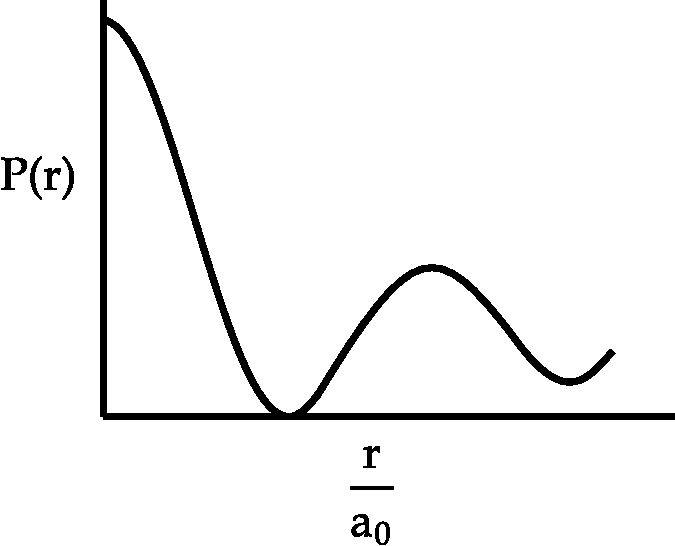
\includegraphics[height=3cm,width=5cm]{diagram-20210824(2)-crop}
		
	\end{figure}
	\task[\textbf{B.}]\begin{figure}[H]
		\centering
		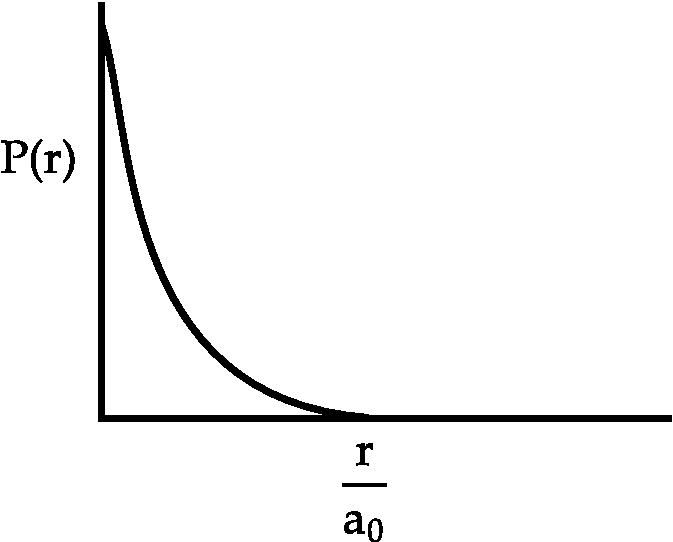
\includegraphics[height=3cm,width=5cm]{diagram-20210824(3)-crop}
		
	\end{figure}
	\task[\textbf{C.}]\begin{figure}[H]
		\centering
		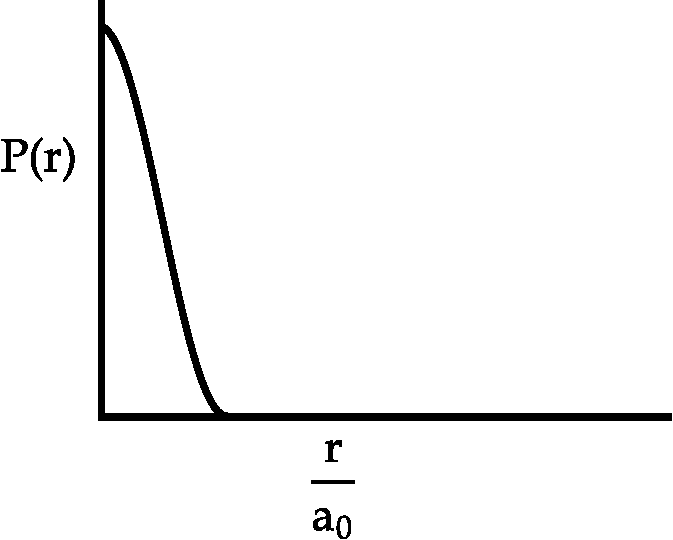
\includegraphics[height=3cm,width=5cm]{diagram-20210824(4)-crop}
		
	\end{figure}
	\task[\textbf{D.}]\begin{figure}[H]
		\centering
		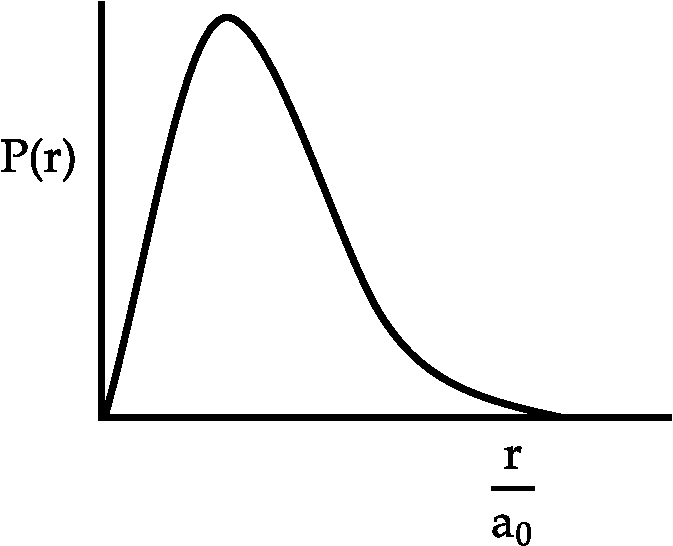
\includegraphics[height=3cm,width=5cm]{diagram-20210824(5)-crop}
	\end{figure}
\end{tasks}
\begin{minipage}{\textwidth}
	\item An electron in the ground state of the hydrogen atom has the wave function $\psi(\vec{r})=\frac{1}{\sqrt{\pi a_{0}^{3}}} e^{-\left(\frac{r}{a_{0}}\right)}$, where $a_{0}$ is constant. The expectation value of the operator $\hat{Q}=z^{2}-r^{2}$, where $z=r \cos \theta$ is
	(Hint: $\left.\int_{0}^{\infty} e^{-a r} r^{n} d r=\frac{\sqrt{n}}{a^{n+1}}=\frac{(n-1) !}{a^{n+1}}\right)$
	\exyear{GATE 2014}
\end{minipage}
\begin{tasks}(4)
	\task[\textbf{A.}] $\frac{-a_{0}^{2}}{2}$
	\task[\textbf{B.}]$-a_{0}^{2}$
	\task[\textbf{C.}]$\frac{-3 a_{0}^{2}}{2}$
	\task[\textbf{D.}]$-2 a_{0}^{2}$
\end{tasks}
\begin{minipage}{\textwidth}
	\item A hydrogen atom is in the state
	$$
	\psi=\sqrt{\frac{8}{21}} \psi_{200}-\sqrt{\frac{3}{7}} \psi_{310}+\sqrt{\frac{4}{21}} \psi_{321},
	$$
	where $n, l, m$ in $\psi_{n l m}$ denote the principal, orbital and magnetic quantum numbers, respectively. If $\vec{L}$ is the angular momentum operator, then the average value of $L^{2}$ is $\cdots \quad \hbar^{2}$
	\exyear{GATE 2014}
\end{minipage}
\begin{minipage}{\textwidth}
	\item An electric field $\vec{E}=E_{0} \hat{z}$ is applied to a Hydrogen atom in $n=2$ excited state. Ignoring spin the $n=2$ state is fourfold degenerate, which in the $|l, m\rangle$ basis are given by $|0,0\rangle,|1,1\rangle,|1,0\rangle$ and $|1,-1\rangle$. If $H^{\prime}$ is the interaction Hamiltonian corresponding to the applied electric field, which of the following matrix elements is nonzero?
	\exyear{GATE 2019}
\end{minipage}
\end{enumerate}


\colorlet{ocre1}{ocre!70!}
\colorlet{ocrel}{ocre!30!}
\setlength\arrayrulewidth{1pt}
\begin{table}[H]
	\centering
	\arrayrulecolor{ocre}
	
	\begin{tabular}{|p{1.5cm}|p{1.5cm}||p{1.5cm}|p{1.5cm}|}
		\hline
		\multicolumn{4}{|c|}{\textbf{Answer key}}\\\hline\hline
		\rowcolor{ocrel}Q.No.&Answer&Q.No.&Answer\\\hline
		1&\textbf{d}&2&\textbf{d}\\\hline
		3&\textbf{d}&4&\textbf{2}\\\hline
		5&\textbf{c}&&\\\hline
	\end{tabular}
\end{table}


\newpage
\begin{abox}
	Practice set 3
	\end{abox}
\begin{enumerate}
	\begin{minipage}{\textwidth}
	\item $\text { Verify that the average value of } 1 / r \text { for a } 1 \text { s electron in the hydrogen atom is } 1 / a_{0} \text {. }$
\end{minipage}
	\begin{answer}
		The wave function of a ls electron is,
		$$
		\psi=\frac{e^{-r / a_{0}}}{\sqrt{\pi} a_{0}^{3 / 2}}
		$$
		Since $d V=r^{2} \sin \theta d r d \theta d \phi$ we have for the expectation value of $1 / r$
		$$
		\begin{aligned}
		\left\langle\frac{1}{r}\right\rangle &=\int_{0}^{\infty}\left(\frac{1}{r}\right)|\psi|^{2} d V \\
		&=\frac{1}{\pi a_{0}^{3}} \int_{0}^{\infty} r e^{-2 r / a_{0}} d r \int_{0}^{\pi} \sin \theta d \theta \int_{0}^{2 \pi} d \phi
		\end{aligned}
		$$
		The integrals have the respective values
		$$
		\begin{gathered}
		\int_{0}^{\infty} r e^{-2 r / a_{0}} d r=\left[\frac{a_{0}^{2}}{4} e^{-2 r / a_{0}}-\frac{r}{2} e^{-2 r / a_{0}}\right]_{0}^{\infty}=\frac{a_{0}^{2}}{4} \\
		\int_{0}^{\pi} \sin \theta d \theta=[-\cos \theta]_{0}^{\pi}=2 \\
		\int_{0}^{2 \pi} d \phi=[\phi]_{0}^{2 \pi}=2 \pi \\
		\left\langle\frac{1}{r}\right\rangle=\left(\frac{1}{\pi a_{0}^{3}}\right)\left(\frac{a_{0}^{2}}{4}\right)(2)(2 \pi)=\frac{1}{a_{0}}
		\end{gathered}
		$$	
	\end{answer}
		\begin{minipage}{\textwidth}
		\item 	Show that the most probable distance by the electron from the nucleus in the ground state of hydrogen atom is equal to the Bohr's radius.
	\end{minipage}
	\begin{answer}
		For the ground state of hydrogen atom, $n=1, \ell=0$ and $m=0$. Hence the ground state wave function is,
		$$
		\psi_{1,0,0}=\left(\frac{1}{\pi a_{0}^{3}}\right)^{1 / 2} e^{-r / a_{0}}
		$$
		Since, the wave function is independent of $\theta$ and $\phi$, therefore,\\
		Radial probability density $=P(r)=\left|\psi_{100}\right|^{2} 4 \pi r^{2}=\frac{4}{a_{0}^{3}} e^{-2 r / a_{0}} r^{2}$
		For most probable distance, $P(r)$ is to be the maximum
		$$
		\frac{d P}{d r}=\frac{4}{a_{0}^{3}}\left[r^{2}\left(-\frac{2}{a_{0}}\right) e^{-2 r / a_{0}}+2 r e^{-2 r / a_{0}}\right]=0 \Rightarrow r=a_{0}
		$$
		Thus the most probable distance of the electron from the nucleus of hydrogen atom in the ground state is equal tothe Bohr radius $\left(a_{0}\right)$.	
	\end{answer}
		\begin{minipage}{\textwidth}
		\item If the ground state wave function for the hydrogen atom is
		$$
		\psi=\frac{1}{\sqrt{\pi}} \frac{1}{a_{0}^{3 / 2}} e^{-r / a_{0}}
		$$
		show that average distance of the electron from the nucleus is $1.5 \mathrm{a}_{0}$.
	\end{minipage}
	\begin{answer}
		We have the average distance of the electron from the hydrogen nucleus in the ground state is,
		$$
		\begin{aligned}
		\langle r\rangle &=\int_{0}^{\infty} \psi^{*} \hat{r} \psi d r=\int_{0}^{\infty} \frac{1}{\sqrt{\pi}} \frac{1}{a_{0}^{3 / 2}} e^{-r / a_{0}} r \frac{1}{\sqrt{\pi}} \frac{1}{a_{0}^{3 / 2}} e^{-r / a_{0}} d \tau \\
		&=\frac{1}{\pi a_{0}^{3}} \int_{0}^{\infty} r e^{-2 r / a_{0}} r^{2} \sin \theta d r d \theta d \phi
		\end{aligned}
		$$
		Using the standard integral $\int_{0}^{\infty} e^{-a x} x^{n} d x=\frac{n !}{a^{n+1}}$, we get
		$$
		\langle r\rangle=\frac{1}{\pi a_{0}^{3}} \int_{0}^{\infty} r^{3} e^{-2 r / a_{0}} d r \int_{0}^{\pi} \sin \theta d \theta \int_{0}^{2 \pi} d \phi=\frac{1}{\pi a_{0}^{3}} \times \frac{3 !}{\left(2 / a_{0}\right)^{4}} \times 2 \times 2 \pi
		$$
		Therefore, $\langle r\rangle=\frac{3}{2} a_{0}=1.5 a_{0}$
	\end{answer}
		\begin{minipage}{\textwidth}
		\item What is the expectation value of the knetice nergy $\left(E^{2}\right)$ of the electron in the 1s state of the hydrogen atom?
	\end{minipage}
	\begin{answer}
		The expectation value of the kinetic energy is,
		$$
		\left\langle E_{k}\right\rangle=\int_{\tau} \psi_{1,0,0}^{*} \hat{E}_{k} \psi_{1,0,0} d \tau=\int_{0}^{\infty} \int_{0}^{\pi} \int_{0}^{2 \pi} \psi_{1,0,0} \hat{E}_{k} \psi_{1,0,0} r^{2} \sin \theta d r d \theta d \phi
		$$
		But, $\quad \vec{E}_{k}=-\frac{\hbar^{2}}{2 m} \nabla^{2}=-\frac{\hbar^{2}}{2 m}\left[\frac{1}{r^{2}} \frac{\partial}{\partial r} r^{2} \frac{\partial}{\partial r}+\frac{1}{r^{2} \sin \theta} \frac{\partial}{\partial \theta} \sin \theta \frac{\partial}{\partial \theta}+\frac{1}{r^{2} \sin ^{2} \theta} \frac{\partial^{2}}{\partial \phi^{2}}\right]$\\
		Since $\psi_{1,0,0}$ depends on $r$ only, the terms in $\frac{\partial}{\partial \theta}$ and $\frac{\partial}{\partial \phi}$ are zero.\\
		$$\left\langle E_{k}\right\rangle=-\frac{\hbar^{2}}{2 m} \cdot 4 \pi\left(\frac{1}{\sqrt{\pi} a_{0}^{3}}\right)^{2} \int_{0}^{\infty} e^{-r / a_{0}} \times\left\{\left(\frac{\partial^{2}}{\partial r^{2}}+\frac{2}{r} \frac{\partial}{\partial r}\right) e^{-r / a_{0}}\right\} r^{2} d r$$
		$$\begin{aligned}
		&=-\frac{\hbar^{2}}{2 m} \frac{4}{a_{0}^{3}} \int_{0}^{\infty}\left(\frac{1}{a_{0}^{2}}-\frac{2}{r a_{0}}\right) e^{-2 r / a_{0}} r^{2} d r \\
		&=-\frac{2 \hbar^{2}}{m a_{0}^{3}}\left[\frac{1}{a_{0}^{2}} \int_{0}^{\infty} r^{2} e^{-2 r / a_{0}} d r-\frac{2}{a_{0}} \int_{0}^{\infty} r e^{-2 r / a_{0}} d r\right] \\
		&=-\frac{2 \hbar^{2}}{m a_{0}^{3}}\left[\frac{1}{a_{0}^{2}} \frac{2}{\left(2 / a_{0}\right)^{3}}-\frac{2}{a_{0}} \frac{1}{\left(2 / a_{0}\right)^{2}}\right]=\frac{2 \hbar^{2}}{m a_{0}^{3}} \cdot \frac{a_{0}}{4}
		\end{aligned}$$
		$\text { Therefore, }\left\langle E_{k}\right\rangle=\frac{\hbar^{2}}{2 m a_{0}^{3}}=\frac{\hbar^{2}}{2 m}\left(\frac{m e^{2}}{\hbar^{2}}\right)=\frac{m e^{4}}{2 \hbar^{2}}$
	\end{answer}
	\begin{minipage}{\textwidth}
	\item Estimate the uncertainity in the radial position of the electron in the ground state of hydrogen atom.
\end{minipage}
	\begin{answer}
		For ground state\\
		$$\langle r \rangle =\frac{4}{a_0^3}	\int_{0}^{\infty} r^3 e^{\frac{-2r}{a_0}}dr=\frac{3a_0}{2}$$
		$$\langle r^2 \rangle =\frac{4}{a_0^3}	\int_{0}^{\infty} r^4 e^{\frac{-2r}{a_0}}dr=3a_0^2$$
		uncertainity in the radial position of the particle will be \\
		$$\Delta r=\sqrt{\langle r^2 \rangle-\langle r \rangle^2}=\frac{\sqrt{3}}{2}a_0$$
	\end{answer}
	\begin{minipage}{\textwidth}
	\item 	Find the positions of maxima of the radial probability curves for 1s,2s,2p and 3d orbitals of the hydrogen like atom 
\end{minipage}
	\begin{answer}
		The radial probability density \\
		$$P_{nl}=r^2|R_{nl}|^2$$
		$$R_{10}=Constant \times e^{-Zr/a_0}$$
		$$R_{21}=Constant \times e^{-Zr/2a_0}$$
		$$R_{32}=Constant \times e^{-Zr/3a_0}$$
		$P_{nl}$ will be maximum when $\frac{dP_{nl}}{dr}=0$ hence \\
		$$\frac{dP_{10}}{dr}=0 \implies C(2r-\frac{2Zr^2}{a_0})e^{\frac{-2Zr}{a_0}}=0$$
		$$\implies r=\frac{a_0}{Z}$$
		$$\frac{dP{21}}{dr}=0\implies C(4r^3-\frac{Zr^4}{a_0})e^{\frac{-Zr}{a_0}}=0$$
		$$\implies r=\frac{4a_0}{Z}$$
		Similarly $\frac{dP_{32}}{dr}=0\implies r=\frac{9a_0}{2}$\\
		In general $r_{max}=\frac{n^2a_0}{2}$
	\end{answer}
		\begin{minipage}{\textwidth}
		\item 	At time $t=0$, the wave function for the hydrogen atom is
		$$
		\psi(r, 0)=\frac{1}{\sqrt{10}}\left(2 \psi_{100}+\psi_{210}+\sqrt{2} \psi_{211}+\sqrt{3} \psi_{21,-1}\right)
		$$
		where the subscripts are values of the quantum numbers $n, l, m$. (i) What is the expectation value for the energy of the system? (ii) What is the probability of finding the system with $l=1, m=1$ ? .
	\end{minipage}
	\begin{answer}
		Expectation value $=\langle E \rangle =\langle \psi |H|\psi\rangle$\\
		$$=\frac{1}{10}\left\langle \left(2 \psi_{100}+\psi_{210}+\sqrt{2} \psi_{211}+\sqrt{3} \psi_{21,-1}\right)|H|\left(2 \psi_{100}+\psi_{210}+\sqrt{2} \psi_{211}+\sqrt{3} \psi_{21,-1}\right)\right\rangle $$
		$$=\frac{1}{10}\left\langle \left(2 \psi_{100}+\psi_{210}+\sqrt{2} \psi_{211}+\sqrt{3} \psi_{21,-1}\right)|\left(2E_1 \psi_{100}+E_2\psi_{210}+\sqrt{2} E_2\psi_{211}+\sqrt{3}E_2 \psi_{21,-1}\right)\right\rangle $$
		$$=\frac{1}{10}\left( 4E_1+E_2+2E_2+3E_2\right) =\frac{1}{10}\left[ 4E_1+6E_2\right] $$
		$$E_1=-13.6eV \quad E_2=-3.4eV$$
		$$\langle E \rangle=-74.8eV$$
	\end{answer}
	\begin{minipage}{\textwidth}
	\item Let $\psi_{n l m}$ denote the eigenfunctions of a Hamiltonian for a spherically symmetric potential $V(r)$
	$$
	\psi_{n, l, m}=\frac{1}{6}\left[\psi_{200}+\sqrt{5} \psi_{210}+\sqrt{10} \psi_{21-1}+\sqrt{20} \psi_{211}\right]
	$$
	Then find
	(a) the expectation value of $L_{z}$\\
	(b) the expectation value of $L^{2}$ in the state\\
	(c) the expectation value of $L_{y}$
\end{minipage}
\begin{answer}
	$\psi_{n m m}=\frac{1}{6}\left[\psi_{200}+\sqrt{5} \psi_{210}+\sqrt{10} \psi_{21-1}+\sqrt{20} \psi_{211}\right]$\\
 (a)\begin{align*}
		\left\langle L_{z}\right\rangle &=\frac{1}{36} 0 \hbar+\frac{5}{36} \times 0 \hbar+\frac{10}{36} \times(-1 \hbar)+\frac{20}{36}(1 \hbar) \\
		&=\frac{10}{36} \hbar=\frac{5}{18} \hbar
	\end{align*}
	(b) $\left\langle L^{2}\right\rangle=\frac{1}{36} \times 0 \hbar^{2}+\frac{5}{36} \times\left(2 \hbar^{2}\right)+\frac{10}{36} \times\left(2 \hbar^{2}\right)+\frac{20}{36}\left(2 \hbar^{2}\right)$
	$$
	=\frac{35}{36}\left(2 \hbar^{2}\right)=\frac{35}{18} \hbar^{2}
	$$
	(c) $L_{y}=\frac{L_{+}-L_{-}}{2 i}$
	\begin{align*}
	&\therefore\left\langle L_{y}\right\rangle=\frac{1}{2 i}\left\{\left\langle L_{+}\right\rangle-\left\langle L_{-}\right\rangle\right\} \\
	&L_{+}|\psi\rangle=\frac{\sqrt{5}}{6} \times \sqrt{2} \hbar \psi_{211}+\frac{\sqrt{10}}{6} \times \sqrt{2} \hbar \psi_{210} \\
	&\left\langle\psi\left|L_{+}\right| \psi\right\rangle=\frac{\sqrt{20} \times \sqrt{5} \times \sqrt{2} \hbar}{36}+\frac{\sqrt{10} \times \sqrt{5} \times \sqrt{2} \hbar}{36} \\
	&L_{-}|\psi\rangle=\frac{\sqrt{5}}{6} \times \sqrt{2} \hbar \psi_{21-1}+\frac{\sqrt{20}}{6} \times \sqrt{2} \hbar \psi_{210} \\
	&\left\langle\psi\left|L_{-}\right| \psi\right\rangle=\frac{\sqrt{10} \times \sqrt{5} \times \sqrt{2} \hbar}{36}+\frac{\sqrt{20} \times \sqrt{5} \times \sqrt{2} \hbar}{36} \quad \therefore\left\langle L_{y}\right\rangle=0
	\end{align*}
\end{answer}
\end{enumerate}






































